\documentclass[tikz,border=1mm]{standalone}
\usepackage[T1]{fontenc}
\usepackage{helvet}
\renewcommand{\familydefault}{\sfdefault}
\usepackage{amsmath}
\usepackage{sansmath}
\sansmath
\usetikzlibrary{positioning,arrows.meta,calc,fit}
\definecolor{cont}{HTML}{F4A6A6}\definecolor{contB}{HTML}{C0605F}
\definecolor{even}{HTML}{C9A7E7}\definecolor{evenB}{HTML}{8E68BD}
\definecolor{modu}{HTML}{B5D99C}\definecolor{moduB}{HTML}{6F9F55}
\definecolor{peri}{HTML}{A7C7E7}\definecolor{periB}{HTML}{5F8DBF}
\definecolor{caja}{HTML}{F4F4F4}\definecolor{borde}{HTML}{8A8A8A}\definecolor{nsga}{HTML}{F7E3C0}
\hyphenpenalty=10000 \exhyphenpenalty=10000
\begin{document}
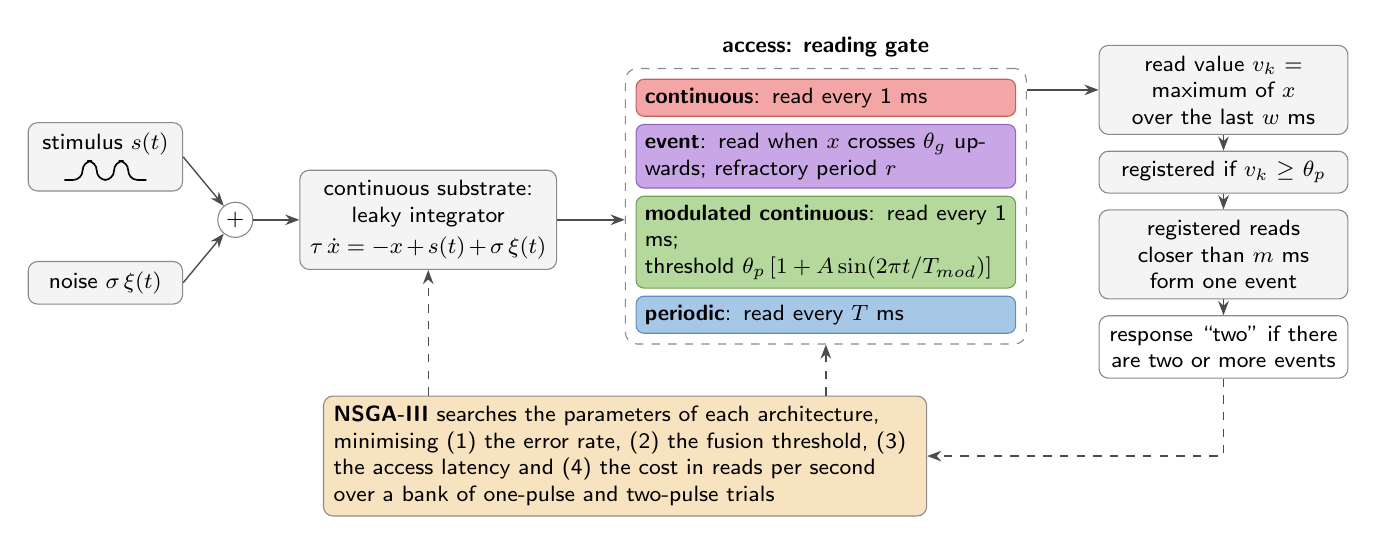
\begin{tikzpicture}[
  >={Stealth[length=1.8mm]}, every node/.style={font=\fontsize{8}{9.6}\selectfont},
  bloque/.style={draw=borde, fill=caja, rounded corners=1.2mm, align=center, inner sep=1.3mm, line width=0.4pt},
  puerta/.style={draw=#1B, fill=#1, rounded corners=1mm, align=left, inner sep=1.1mm, text width=46mm, line width=0.4pt},
  flecha/.style={->, line width=0.5pt, draw=black!70}]
  %% estímulo, ruido e integrador (sustrato continuo)
  \node[bloque, text width=17mm] (est) at (0, 0.8) {stimulus $s(t)$\\[0.6mm]
    \tikz{\draw[line width=0.6pt, line join=miter, line cap=rect] (0,0) -- (0.22,0) -- (0.22,0.24) -- (0.40,0.24) -- (0.40,0) -- (0.62,0) -- (0.62,0.24) -- (0.80,0.24) -- (0.80,0) -- (1.02,0);}};
  \node[bloque, text width=17mm] (rui) at (0, -0.8) {noise $\sigma\,\xi(t)$};
  \node[draw=borde, circle, inner sep=0.5mm, fill=white] (suma) at (1.65, 0) {$+$};
  \draw[flecha] (est.east) -- (suma); \draw[flecha] (rui.east) -- (suma);
  \node[bloque, text width=30mm] (int) at (4.1, 0) {continuous substrate:\\leaky integrator\\[0.6mm]$\tau\,\dot{x}=-x+s(t)+\sigma\,\xi(t)$};
  \draw[flecha] (suma) -- (int);
  %% compuertas de lectura (acceso)
  \node[puerta=cont] (g1) at (9.15, 1.55) {\textbf{continuous}: read every 1 ms};
  \node[puerta=even, below=0.9mm of g1] (g2) {\textbf{event}: read when $x$ crosses $\theta_g$ upwards; refractory period $r$};
  \node[puerta=modu, below=0.9mm of g2] (g3) {\textbf{modulated continuous}: read every 1 ms;\\threshold $\theta_p\,[1+A\sin(2\pi t/T_{mod})]$};
  \node[puerta=peri, below=0.9mm of g3] (g4) {\textbf{periodic}: read every $T$ ms};
  \node[draw=borde, dashed, rounded corners=1.5mm, inner sep=1.3mm, fit=(g1)(g4)] (gates) {};
  \node[font=\fontsize{8}{9.6}\selectfont\bfseries, above=0.2mm of gates] {access: reading gate};
  \draw[flecha] (int.east) -- (gates.west |- int.east);
  %% lectura, registro, fusión y respuesta
  \node[bloque, text width=29mm] (lee) at (14.2, 1.65) {read value $v_k$ = maximum of $x$ over the last $w$ ms};
  \node[bloque, text width=29mm, below=2mm of lee] (reg) {registered if $v_k\ge\theta_p$};
  \node[bloque, text width=29mm, below=2mm of reg] (fus) {registered reads closer than $m$ ms form one event};
  \node[bloque, text width=29mm, below=2mm of fus, fill=white] (res) {response ``two'' if there are two or more events};
  \draw[flecha] (gates.east |- lee.west) -- (lee.west);
  \draw[flecha] (lee) -- (reg); \draw[flecha] (reg) -- (fus); \draw[flecha] (fus) -- (res);
  %% NSGA-III
  \node[bloque, fill=nsga, text width=74mm, align=left] (obj) at (6.6, -3.0) {\textbf{NSGA-III} searches the parameters of each architecture, minimising (1) the error rate, (2) the fusion threshold, (3) the access latency and (4) the cost in reads per second over a bank of one-pulse and two-pulse trials};
  \draw[flecha, dashed] (int.south |- obj.north) -- (int.south);
  \draw[flecha, dashed] (gates.south |- obj.north) -- (gates.south);
  \draw[flecha, dashed] (res.south) |- (obj.east);
\end{tikzpicture}
\end{document}
